\lysh{15474}{4}
\begin{alist}
\item Έχουμε: $P(x) = e^{\ln e}x^3 + 4x^2 \ln\sqrt{e} + 2 = ex^3 + 4x^2 \ln e^{\frac{1}{2}} + 2 = ex^3 + 4x^2 \cdot \frac{1}{2}\ln e + 2 = ex^3 + 2x^2 + 2$.
\item Οι τετμημένες των σημείων τομής της γραφικής παράστασης της πολυωνυμικής συνάρτησης $P(x)$ με την ευθεία $\varepsilon: y = ex + 4$ είναι οι ρίζες της εξίσωσης
\begin{align*}
P(x) - (ex + 4) = 0 &\Leftrightarrow ex^3 + 2x^2 + 2 - ex - 4 = 0 \\
&\Leftrightarrow ex^3 + 2x^2 - ex - 2 = 0 \\
&\Leftrightarrow x^2(ex + 2) - (ex + 2) = 0 \\
&\Leftrightarrow (ex + 2) \cdot (x^2 - 1) = 0.
\end{align*}
Άρα οι τετμημένες των σημείων τομής είναι: $x = 1$, $x = -1$ και $x = -\dfrac{2}{e}$.
\item Για να βρούμε τα διαστήματα του $x$ που η γραφική παράσταση της πολυωνυμικής συνάρτησης $P(x)$ είναι πάνω από την ευθεία $\varepsilon: y = ex + 4$ θα λύσουμε την ανίσωση:
\[P(x) - (ex + 4) > 0 \Leftrightarrow (ex + 2) \cdot (x^2 - 1) > 0.\]
Οι ρίζες του $(ex + 2) \cdot (x^2 - 1)$ είναι $x = 1$, $x = -1$ και $x = -\dfrac{2}{e}$. \\
Το πρόσημο του $(ex + 2) \cdot (x^2 - 1)$ φαίνεται στον παρακάτω πίνακα:
\begin{center}
\begin{tikzpicture}
\tkzTabInit[color,lgt=3,espcl=2,colorC = maincolor!40,
colorL = maincolor!20,
colorV = maincolor!40]%
  {$x$ /1, $(ex+2)(x^2-1)$ /.8}
  {$-\infty$, $-1$, $-2/e$, $1$, $+\infty$}
\tkzTabLine{ , -, z, +, z, -, z, +, }
\end{tikzpicture}
\end{center}
Άρα $x \in \left(-1, -\dfrac{2}{e}\right) \cup (1, +\infty)$.
\item Παρατηρούμε ότι το $P(e) - e^2 - 4$ είναι η τιμή του $P(x) - (ex + 4)$ για $x = e$. \\
Σύμφωνα με το προηγούμενο ερώτημα θα έχουμε $P(e) - e^2 - 4 > 0$, αφού $e > 1$.
\end{alist}

